\subsection{On confidence intervals}

Figure \ref{fig:ci} details the impact of our diversion policy for the 3 site
case with a 60 minute lead time (this is essentially the same
curve for the 60 minute lead time as in the first plot of Figure
\ref{fig:3sites_all}). The confidence intervals show that
the positive impact of our diversion policy is statistically
significant. Also, note that as we increase the fraction of
volunteers, the variance also increases. The reason is that,
when there are more volunteers, there are more diversions which
induce greater variance. If we examine performance improvment
for other metrics or for other levels of granularity, similar patterns
can be observed.

\begin{figure}[htp]
\centering
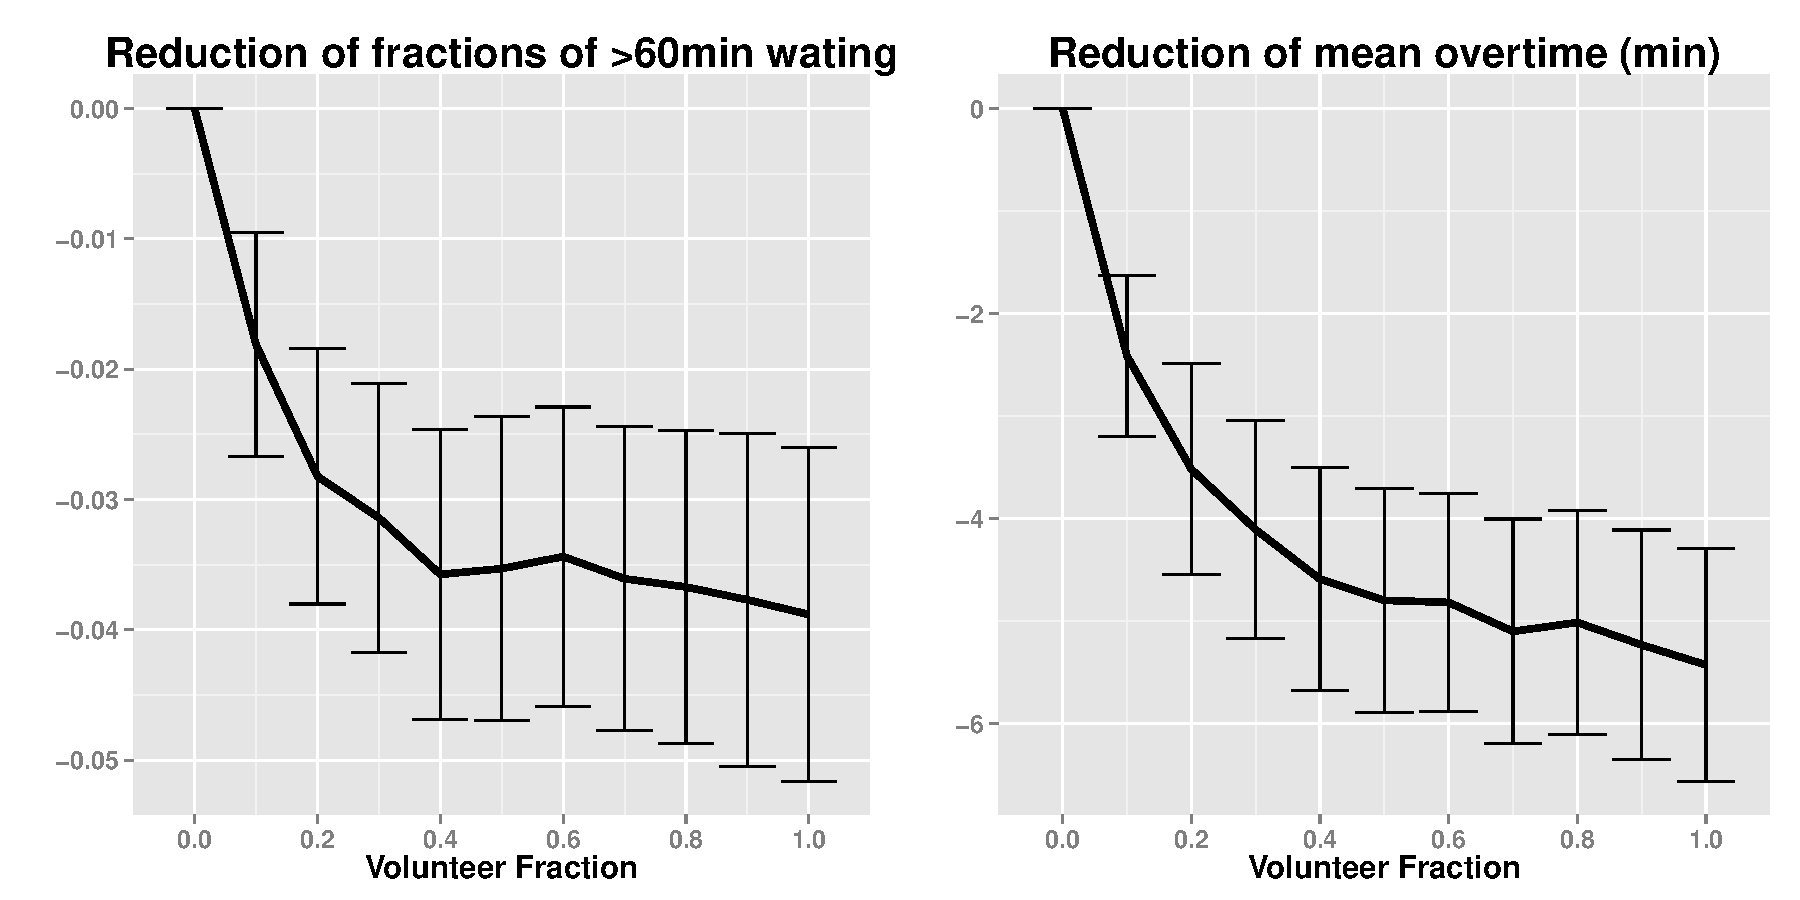
\includegraphics[width=.6\textwidth]{chap3/numeric/pic/ci}
\caption{The improvement for the fraction of over 60 minute waiting
for the 3 site case with a 60 minute lead time.}
\label{fig:ci}
\end{figure}
